\documentclass[12pt]{article}
\usepackage{amsmath}
\usepackage{multirow}
\usepackage{enumerate}
\usepackage{graphicx}
\usepackage{changepage}
\usepackage[all]{xy}
\usepackage{tikz}
\usetikzlibrary{shapes}


\setlength{\voffset}{-3cm}
%\setlength{\hoffset}{-2cm}
%\setlength{\parindent}{0cm}
\setlength{\textheight}{26cm}
%\setlength{\textwidth}{14cm}


\begin{document}


\begin{center}

\includegraphics[width=0.6\textwidth]{ul_logo}
\quad\\[1cm]
{\bf\large FACULTY OF SCIENCE AND ENGINEERING\\[0.5cm]}
{\bf\small DEPARTMENT OF MATHEMATICS AND STATISTICS\\[0.8cm]}
{\large END OF SEMESTER ASSESSMENT PAPER\\[2cm]}
\begin{adjustwidth}{-1cm}{0cm}
\begin{tabular}{l@{\qquad}l}
MODULE CODE: MA4413&SEMESTER: Autumn 2014\\[1cm]
MODULE TITLE: Statistics for Computing& DURATION OF EXAM: 2.5 hours\\[1cm]
LECTURER: Dr.~Kevin Burke& GRADING SCHEME: 100 marks \\
& \hspace{3cm} (60\% of module)\\[2cm]
%EXTERNAL EXAMINER:&\\
%Prof. Brendan Murphy&\\[1cm]
\end{tabular}
\end{adjustwidth}
{\bf INSTRUCTIONS TO CANDIDATE}
\end{center}
\begin{small}
\begin{itemize}\itemsep0.3cm
\item {\bf Attempt four} of the six questions (each one carries 25 marks).
\item All work must be shown \emph{clearly and logically} using appropriate symbols and probability notation. Failure to do so will \emph{lose marks}.
\item Write down the formula you intend to use at each stage \emph{before} filling it in with numbers.
\item Formula sheets are provided at the back of this exam paper.
\item Statistical tables are available from the invigilators.
\end{itemize}
\end{small}
\newpage

\section*{Question 1 \qquad{\small(25 Marks)}}
\noindent\rule{\linewidth}{1pt}
\quad\\[-0.5cm]
\begin{enumerate}[a)]
\item We wish to investigate the battery life for two types of laptop. Eight Type A and eight Type B laptops were fully charged and then run until the batteries reached a critical level. In each case the time (in hours) was recorded and the results were as follows:\\[-0.6cm]
    \begin{center}
    \begin{tabular}{|c|cccccccc|}
    \hline
    &&&&&&&&\\[-0.3cm]
    Type A & 2.7 & 2.9 & 4.1 & 4.3 & 5.7 & 6.6 & 9.0 & 15.0  \\[0.1cm]
    \hline
    &&&&&&&&\\[-0.3cm]
    Type B & 1.0 & 1.0 & 1.8 & 2.3 & 2.3 & 3.3 & 3.5 & 5.5 \\[0.1cm]
    \hline
    \end{tabular}
    \end{center}
    \begin{enumerate}[i)]\itemsep0.3cm
    %\item Calculate the mean battery life for each type. \hfill{\scriptsize \bf (2 marks)}
    \item Find the values of $Q_1$, $Q_2$ and $Q_3$ for each type. \hfill{\scriptsize \bf (3 marks)}
    \item Identify any outliers in each group. \hfill{\scriptsize \bf (2 marks)}
    \item Draw the boxplots for each type side by side. \hfill{\scriptsize \bf (3 marks)}
    \item Comment on the boxplots. \hfill{\scriptsize \bf (2 marks)}
    \end{enumerate}
\begin{center}\noindent\rule{0.4\linewidth}{0.5pt}\end{center}
\item Identify the data type for each of the following quantities:
    \begin{enumerate}[i)]\itemsep0.3cm
    \item laptop battery life\,; \hfill{\scriptsize \bf (1 mark)}
    \item age group  (``$18-22$'', ``$23-30$'', ``$30+$'')\,; \hfill{\scriptsize \bf (1 mark)}
    \item the number of lines of code in a program\,; \hfill{\scriptsize \bf (1 mark)}
    \item gender\,;\hfill{\scriptsize \bf (1 mark)}
    \item temperature. \hfill{\scriptsize \bf (1 mark)}
    \end{enumerate}
    \begin{center}\noindent\rule{0.4\linewidth}{0.5pt}\end{center}
\item A bottle-filling machine is programmed to put 500ml into each bottle. To test if the machine is working correctly, a sample of 40 bottles was selected and, for this sample, the average content was 501.5ml and the standard deviation was 3.05 ml.
    \begin{enumerate}[i)]\itemsep0.3cm
    \item What is the parameter here? (provide symbol and value) \hfill{\scriptsize \bf (2 marks)}
    \item What is the statistic here? (provide symbol and value) \hfill{\scriptsize \bf (2 marks)}
    \item Calculate a 95\% confidence interval for the parameter; does the evidence suggest that the machine is working as programmed? \hfill{\mbox{\scriptsize \bf (3 marks)}}
    \item How large a sample is required to reduce the margin of error in the previous confidence interval to $\pm0.5$ml? \hfill{\scriptsize \bf (3 marks)}
    \end{enumerate}
\end{enumerate}
\quad\\[-0.3cm]
\noindent\rule{\linewidth}{1pt}

\newpage

\section*{Question 2 \qquad{\small(25 Marks)}}
\noindent\rule{\linewidth}{1pt}
\quad\\[-0.5cm]
\begin{enumerate}[a)]
\item Consider the following sample of incomes (in thousands) of 40 individuals living in a particular area:\\[-0.6cm]
    \begin{center}
    \begin{tabular}{|cccccccccc|}
    \hline
    &&&&&&&&&\\[-0.3cm]
    14 & 14 & 15 & 15 & 15 & 15 & 15 & 15 & 15 & 15 \\[0.1cm]
    15 & 15 & 16 & 18 & 19 & 19 & 19 & 20 & 21 & 21 \\[0.1cm]
    22 & 22 & 24 & 24 & 24 & 26 & 27 & 28 & 29 & 33 \\[0.1cm]
    36 & 38 & 38 & 39 & 41 & 44 & 44 & 45 & 48 & 71 \\[0.1cm]
    \hline
    \end{tabular}
    \end{center}
    \begin{enumerate}[i)]\itemsep0.3cm
    \item Construct a frequency table with 6 classes (note: use 12 as the first breakpoint when setting up the intervals).\hfill{\mbox{\scriptsize \bf (4 marks)}}
    %\item Add a column of relative frequencies and, hence, estimate the proportion of individuals earning between 22000 and 42000. \hfill{\mbox{\scriptsize \bf (2 marks)}}
%    \item Based on the frequency table, estimate the proportion of individuals earning between 22000 and 42000. \hfill{\mbox{\scriptsize \bf (1 mark)}}
    \item Draw the histogram. \hfill{\scriptsize \bf (3 marks)}
    \item What measure of centrality is appropriate for this data? Calculate its value. \hfill{\scriptsize \bf (3 marks)}
    \end{enumerate}
\begin{center}\noindent\rule{0.4\linewidth}{0.5pt}\end{center}
\item A manufacturer wants to compare two designs of CPU in terms of clock speed. Two small samples are selected and the results are as follows:
\begin{small}
\begin{center}
\begin{tabular}{|c|c|c|}
\hline
&&\\[-0.3cm]
& Design 1 & Design 2 \\
\hline
&&\\[-0.2cm]
sample size      & 8 & 12 \\[0.2cm]
mean   & 1.211\,\,Ghz  & 0.870\,\,Ghz \\[0.2cm]
variance &  0.05\,\,Ghz$^2$ & 0.04\,\,Ghz$^2$ \\[0.2cm]
\hline
\end{tabular}
\end{center}
\end{small}
\begin{enumerate}[i)]\itemsep0.6cm
    \item Before comparing means, \texttt{var.test} was carried out using \texttt{R}:\\[0.2cm]
\begin{footnotesize}
\begin{tabular}{|l|}
\hline
\texttt{            F test to compare two variances} \\
\texttt{F = 1.243, num df = 7, denom df = 11, p-value = 0.7168}\\
\texttt{alternative hypothesis: true ratio of variances is not equal to 1}\\
\hline
\multicolumn{1}{c}{}
\end{tabular}
\end{footnotesize}
State $H_0$ and $H_a$ for this test. Based on the above output, provide your conclusion (this impacts your calculations for part (ii)).    \hfill{\mbox{\scriptsize \bf (3 marks)}}
    \item Formally test the hypothesis that there is no difference in the mean clock speeds for the two CPU designs using the 1\% level of \mbox{significance:}\\[0.15cm]
        $\bullet$\quad Write down $H_0$ and $H_a$.\\[0.15cm]
        $\bullet$\quad Compute the test statistic (equal or non-equal variance approach?).\\[0.15cm]
        $\bullet$\quad Compare this test statistic to the appropriate critical value.\\[0.15cm]
        $\bullet$\quad Conclusion: statistical \emph{and} non-statistical language.
     \hfill{\scriptsize \bf (10 marks)}
     \item The t-test requires the data to be approximately normally distributed. What plot is used to check this? Draw a rough picture of what such a plot looks like. \hfill{\mbox{\scriptsize \bf (2 marks)}}
    \end{enumerate}
\end{enumerate}
\quad\\[-0.3cm]
\noindent\rule{\linewidth}{1pt}

\newpage



\section*{Question 3 \qquad{\small(25 Marks)}}
\noindent\rule{\linewidth}{1pt}
\quad\\[-0.5cm]
\begin{enumerate}[a)]
\item A sample of employees was randomly selected. Each of them was assigned the same task of programming a procedure using C++. The number of lines of code used in each case was recorded:
\begin{center}
\begin{tabular}{|ccccc|}
\hline
&&&&\\[-0.4cm]
13 & 9 & 8 & 10 & 5\\
\hline
%\multicolumn{6}{c}{}
\end{tabular}
\end{center}
Calculate the following for the above sample:
    \begin{enumerate}[i)]\itemsep0.3cm
%    \item The median. \hfill{\scriptsize \bf (1 mark)}
    \item the mean\,; \hfill{\scriptsize \bf (1 mark)}
    \item the variance\,; \hfill{\scriptsize \bf (2 marks)}
    \item the standard deviation\,; \hfill{\scriptsize \bf (1 mark)}
    \item a 90\% confidence interval for the true mean. \hfill{\scriptsize \bf (3 marks)}
%    \item Finally, describe \emph{briefly} what a confidence interval is. \hfill{\scriptsize \bf (2 marks)}
    \end{enumerate}
\begin{center}\noindent\rule{0.4\linewidth}{0.5pt}\end{center}
\item Let $\Pr(A) = 0.4$, $\Pr(B)=0.8$ and $\Pr(A\cap B) = 0.3$.\\[0.2cm]
    Calculate the following:
    \begin{enumerate}[i)]\itemsep0.3cm
    \item $\Pr(A\cup B)$\,; \hfill{\scriptsize \bf (1 mark)}
    \item $\Pr(B\,|\,A)$\,; \hfill{\scriptsize \bf (1 mark)}
    \item $\Pr(A^c \cup B^c)$. \hfill{\scriptsize \bf (1 mark)}
%    \item Show that $A$ and $B$ are \emph{not} independent events.\hfill{\scriptsize \bf (1 mark)}
    \end{enumerate}
    \begin{center}\noindent\rule{0.4\linewidth}{0.5pt}\end{center}
\item Assume that a manufacturer of laptops sources processors from two different companies: $C_1$ and $C_2$. Specifically, 80\% of stock comes from $C_1$ and the rest comes from $C_2$.\\[0.2cm]
    Let $X$ be the temperature of a CPU after one hour of moderate use.\\[0.3cm]
     For a $C_1$ processor the temperature is $\text{Normal}(\mu_1=30,\sigma_1 = 1)$.\\[0.3cm]
    For a $C_2$ processor the temperature is $\text{Normal}(\mu_2=29,\sigma_2 = 5)$.\\[-0.2cm]
    \begin{enumerate}[i)]\itemsep0.4cm
%    \item What is the value of $\Pr(C_2)$? \hfill{\scriptsize \bf (1 mark)}
    \item Show that (rounding to two decimal places): \\[0.2cm]
        $\bullet$\quad$\Pr(X>31\,|\,C_1) = 0.16$ and \\[0.2cm]
        $\bullet$\quad$\Pr(X>31\,|\,C_2) = 0.34$. \hfill{\scriptsize \bf (4 marks)}
    %    \item Show that $\Pr(X>31\,|\,C_2) = 0.3446$. \hfill{\scriptsize \bf (2 marks)}
    \item Calculate $\Pr(X>31\cap C_1)$ and $\Pr(X>31\cap C_2)$. \hfill{\scriptsize \bf (4 marks)}
    \item Calculate $\Pr(X>31)$ using the law of total probability. \hfill{\scriptsize \bf (3 marks)}
    \item Calculate $\Pr(C_1\,|\,X<31)$. \hfill{\scriptsize \bf (4 marks)}
    \end{enumerate}
\end{enumerate}
\quad\\[-0.3cm]
\noindent\rule{\linewidth}{1pt}

\newpage




\section*{Question 4 \qquad{\small(25 Marks)}}
\noindent\rule{\linewidth}{1pt}
\quad\\[-0.5cm]
\begin{enumerate}[a)]
\item Consider a RAID-1 (redundant array of inexpensive disks) system constructed using two hard disks that work/fail \emph{independently} of each other. Let $H_1 =$ ``hard disk 1 works'' and $H_2 =$ ``hard disk 2 works'' and, furthermore, $\Pr(H_1) = \Pr(H_2) = 0.2$, i.e., these hard disks are of a very low quality (20\% chance of working).
    \begin{enumerate}[i)]\itemsep0.3cm
    \item Calculate $\Pr(\text{RAID-1 fails})$. Note that a RAID-1 system will only fail if \emph{both} hard disks fail. \hfill{\scriptsize \bf (2 marks)}
    \item How many hard disks are required to reduce the failure  probability, $\Pr(\text{RAID-1 fails})$, to 0.01? \hfill{\scriptsize \bf (3 marks)}
    \end{enumerate}
\begin{center}\noindent\rule{0.4\linewidth}{0.5pt}\end{center}
\item Assume that 10\% of all audio cables produced by a particular company are defective in some way. Thus, if defects occur independently of one another, the number of defective cables in a shipment of size $n$ has a binomial distribution, i.e., $X \sim \text{Binomial}(n,p)$.\\[0.3cm]
    Calculate:
    \begin{enumerate}[i)]\itemsep0.3cm
    \item the probability that there are at least 2 defective cables in a shipment of size 10\,; \hfill{\mbox{\scriptsize \bf (3 marks)}}
    \item the probability that there are less than 15 defective cables in a shipment of size 100\,; \hfill{\mbox{\scriptsize \bf (3 marks)}}
    \item the expected number of defective cables in a shipment of size 20 and the corresponding standard deviation. \hfill{\scriptsize \bf (3 marks)}
    \end{enumerate}
    \begin{center}\noindent\rule{0.4\linewidth}{0.5pt}\end{center}
\item Emails arrive at a rate of 4 per hour according to a Poisson distribution.\\[0.3cm]
    Calculate:
    \begin{enumerate}[i)]\itemsep0.3cm
    \item the probability of receiving exactly 4 emails in a one-hour period\,; \phantom{aaa}\hfill{\mbox{\scriptsize \bf (2 marks)}}
    \item the probability of receiving between 2 and 4 emails in \emph{half} an hour\,; \phantom{a} \hfill{\scriptsize \bf (3 marks)}
    \item the probability of receiving between 10 and 20 emails in a five-hour period\,; \phantom{a} \hfill{\scriptsize \bf (3 marks)}
    \item the probability that the \emph{waiting time} until the next email is greater than 30 minutes. \hfill{\scriptsize \bf (3 marks)}
%    \item The expected waiting time. \phantom{a}  \hfill{\scriptsize \bf (3 marks)}
    \end{enumerate}
\end{enumerate}
\quad\\[-0.3cm]
\noindent\rule{\linewidth}{1pt}

\newpage




\section*{Question 5 \qquad{\small(25 Marks)}}
\noindent\rule{\linewidth}{1pt}
\quad\\[-0.5cm]
\begin{enumerate}[a)]
\item Consider the following probability distribution:
\begin{center}
\begin{tabular}{|c|cccc|}
\hline
&&&&\\[-0.4cm]
$x$        & 1 & 3 & 5 & 10 \\
\hline
&&&&\\[-0.4cm]
$\Pr(X=x)$ & ?? & 0.2 & 0.2 & 0.1 \\
\hline
\multicolumn{5}{c}{}
\end{tabular}
\end{center}
Calculate:
    \begin{enumerate}[i)]\itemsep0.2cm
    \item $\Pr(X=1)$\,; \hfill{\scriptsize \bf (1 mark)}
    \item the expected value, $E(X)$, and explain what it means\,; \hfill{\scriptsize \bf (2 marks)}
    \item the standard deviation, $Sd(X)$. \hfill{\scriptsize \bf (2 marks)}
    \end{enumerate}
\begin{center}\noindent\rule{0.4\linewidth}{0.5pt}\end{center}
\item A soft drinks company is working on a new recipe for its best-selling drink. The company intends to carry out a study where participants will taste both flavours (current and new) and then answer the question:
    \begin{quotation}
    ``Do you prefer the new flavour?''
    \end{quotation}
    It is assumed that the \emph{current} recipe is superior, i.e., that \emph{less than or equal to} 50\% of people prefer the new drink ($p \le 0.5$).\\[0.4cm]
    We wish to test the hypothesis that $p \le 0.5$.\\[-0.4cm]
    \begin{enumerate}[i)]\itemsep0.3cm
    \item What type of data will be collected in this study? \hfill{\mbox{\scriptsize \bf (2 marks)}}
    \item State the null and alternative hypotheses. \hfill{\mbox{\scriptsize \bf (2 marks)}}
    \item From a sample of 65 people, we find that 43 people prefer the new recipe. Calculate the test statistic and, hence, the p-value. \hfill{\mbox{\scriptsize \bf (4 marks)}}
    \item Based on the evidence (i.e., the p-value), state your conclusion in both stastical and non-statistical language. \hfill{\scriptsize \bf (2 marks)}
    \end{enumerate}
    \begin{center}\noindent\rule{0.4\linewidth}{0.5pt}\end{center}
\item Let $X \sim \text{Normal}(\mu = 20, \sigma = 3)$.\\[0.3cm]
    Calculate the following:
    \begin{enumerate}[i)]\itemsep0.3cm
    \item $\Pr(X < 25)$\,; \hfill{\scriptsize \bf (3 marks)}
    \item the value $x$ such that $\Pr(X > x) = 0.1$\,; \hfill{\scriptsize \bf (3 marks)}
    \item $\Pr(\,\overline{\!X} > 19.5)$ where $\,\overline{\!X}$ is the sample mean for a group of $n=40$.\\
        \phantom{a}\hfill{\scriptsize \bf (4 marks)}
    %\item $\Pr(X_1 < X_2)$ where $X_1 \sim \text{Normal}(\mu_1 = 20, \sigma_1 = 3)$,\\ \phantom{$\Pr(X_1 < X_2)$}\hspace{0.4cm} and $X_2 \sim \text{Normal}(\mu_2 = 18, \sigma_2 = 2)$. \hfill{\scriptsize \bf (3 marks)}
    \end{enumerate}
\end{enumerate}
\quad\\[-0.3cm]
\noindent\rule{\linewidth}{1pt}

\newpage







\section*{Question 6 \qquad{\small(25 Marks)}}
\noindent\rule{\linewidth}{1pt}
\quad\\[-0.5cm]
\begin{enumerate}[a)]
\item Customers arrive to a service counter at a rate of $\lambda_a=30$ per hour; the average service time is $E(T_s) = 0.025$ hours. Assume that this is an $M/M/1$ system, i.e., the number of arrivals per hour is $X_a \sim \text{Poisson}(\lambda_a)$ and the service time is $T_s \sim \text{Exponential}(\lambda_s)$. Also define:\\[0.2cm]
    \phantom{a}\qquad\qquad$\bullet$\quad $T=$ time spent in the whole system\,;\\[0.2cm]
    \phantom{a}\qquad\qquad$\bullet$\quad  $N=$ number of customers in the whole system\,;\\[0.2cm]
    \phantom{a}\qquad\qquad$\bullet$\quad  $T_q=$ time spent in the queue component\,;\\[0.2cm]
    \phantom{a}\qquad\qquad$\bullet$\quad  $N_q=$ number of customers in the queue component.\\[0.4cm]
    Calculate:
    \begin{enumerate}[i)]\itemsep0.2cm
    \item the service rate\,; \hfill{\scriptsize \bf (2 marks)}
    \item $E(T)$, $E(N)$, $E(T_q)$ and $E(N_q)$\,; \hfill{\mbox{\scriptsize \bf (5 marks)}}
     \item the utilisation factor and interpret its value\,; \hfill{\mbox{\scriptsize \bf (2 marks)}}
     \item the probability that a customer spends less than 12 minutes in the system\,; \hfill{\mbox{\scriptsize \bf (3 marks)}}
     \item the probability that more than 7 customers exit the system in a 10 minute period. \hfill{\mbox{\scriptsize \bf (3 marks)}}
    \end{enumerate}
\begin{center}\noindent\rule{0.4\linewidth}{0.5pt}\end{center}
\item A source file contains only four unique characters as indicated below.\quad
\begin{center}
\begin{tabular}{|c|cccc|}
\hline
&&&&\\[-0.4cm]
$x$        & a & b & c & d \\
\hline
&&&&\\[-0.4cm]
$p(x)$ & 0.5 & 0.25 & 0.2 & 0.05 \\
\hline
\multicolumn{5}{c}{}
\end{tabular}
\end{center}
    \begin{enumerate}[i)]\itemsep0.3cm
    \item Calculate the entropy for this file. \hfill{\mbox{\scriptsize \bf (3 marks)}}
    \item Construct a Huffman code for the characters $\{a,b,c,d\}$. \hfill{\mbox{\scriptsize \bf (3 marks)}}
    \item Calculate the expected length of this Huffman code and, hence, its efficiency. \hfill{\scriptsize \bf (4 marks)}
    \end{enumerate}
    \begin{center}\noindent\rule{0.4\linewidth}{0.5pt}\end{center}
\end{enumerate}
%\quad\\[-0.3cm]
%\noindent\rule{\linewidth}{1pt}

\newpage














\section*{Useful Formulae: Page 1\\[0.3cm]}
{\bf Histogram:}\\[-0.8cm]
\begin{align*}
\bullet\quad \text{class width} = \frac{\max(x) - \min(x)}{\text{number of classes}}\\
\end{align*}
{\bf Numerical Summaries:}\\[-0.8cm]
\begin{align*}
\bullet\quad \bar x &= \frac{\sum\,x_i}{n}\\[0.6cm]
\bullet\quad s^2 &= \frac{\sum\,x_i^2 - n\,\bar x^2}{n-1}\\[0.6cm]
\bullet\quad \text{Position of } Q_k:& \quad \frac{n+1}{4}\times k \\[0.6cm]
\bullet\quad IQR &= Q_3 - Q_1 \\[0.6cm]
\bullet\quad LF &= Q_1 - 1.5 \times IQR \\[0.6cm]
\bullet\quad UF &= Q_3 + 1.5 \times IQR\\
\end{align*}
{\bf Probability:}\\[-0.8cm]
\begin{align*}
\bullet\quad \Pr(A^c) &= 1 - \Pr(A) \\[1cm]
\bullet\quad \Pr(A \cup B) &= \Pr(A) + \Pr(B) - \Pr(A \cap B)\\[0.6cm]
\bullet\quad \Pr(E_1 \cup E_2 \cup \cdots \cup E_k) &= \Pr(E_1) + \Pr(E_2) + \cdots + \Pr(E_k) \text{\quad{\footnotesize(if mutually exclusive)}}\\[1cm]
\bullet\quad \Pr(A \cap B) &= \Pr(A) \, \Pr(B \, | \, A) = \Pr(B) \, \Pr(A \, | \, B) \\[0.6cm]
\bullet\quad \Pr(E_1 \cap E_2 \cap \cdots \cap E_k) &= \Pr(E_1) \, \Pr(E_2) \, \cdots \, \Pr(E_k) \text{\quad{\footnotesize(if independent)}}\\[1cm]
\bullet\quad \Pr(A\,|\,B) &= \frac{\Pr(A \cap B)}{\Pr(B)} = \frac{\Pr(A) \,\Pr(B\,|\,A)}{\Pr(B)}\\[1cm]
\bullet\quad \Pr(B) = \Pr(B \cap E_1) &+ \Pr(B \cap E_2) + \cdots + \Pr(B \cap E_k) \\[0.2cm]
= \Pr(E_1) \, \Pr(B\,|\,&E_1) + \Pr(E_2) \, \Pr(B\,|\,E_2) + \cdots + \Pr(E_k) \, \Pr(B\,|\,E_k)\\[0.1cm]
\text{{\footnotesize(if $E_1,\ldots, E_k$}} & \,\, \text{{\footnotesize are mutually exclusive \& exhaustive)}}
\end{align*}

\newpage

\section*{Useful Formulae: Page 2\\[0.3cm]}
{\bf Counting Techniques:}\\[-0.8cm]
\begin{align*}
\bullet\quad n\,! &= n\times(n-1)\times(n-2)\times\cdots\times3\times2\times 1\\[0.6cm]
\bullet\quad \binom{n}{k} &= \frac{n\,!}{k\,! \,(n-k)\,!}\\
\end{align*}
{\bf Random Variables:}\\[-0.8cm]
\begin{align*}
\bullet\quad E(X) &= \sum x_i \,\, p(x_i)\\[0.6cm]
\bullet\quad E(X^2) &= \sum x_i^2 \,\, p(x_i)\\[0.6cm]
\bullet\quad Var(X) &= E(X^2) - [E(X)]^2\\[0.6cm]
\bullet\quad Sd(X) &= \sqrt{Var(X)}\\
\end{align*}
{\bf Distributions:}\\[-0.0cm]
\begin{adjustwidth}{-2.1cm}{0cm}
\begin{tabular}{|c@{\quad}|c@{\quad}|c@{\quad}|}
\hline
&&\\[-0.3cm]
$\bullet\quad X \sim \text{Binomial}(n,p)$ & $\bullet\quad X \sim \text{Poisson}(\lambda)$ & $\bullet\quad T \sim \text{Exponential}(\lambda)$ \\[0.6cm]
${\displaystyle\bullet\quad \Pr(X=x) = \binom{n}{x}\,p^x\,(1-p)^{n-x}}$ & ${\displaystyle\bullet\quad \Pr(X=x) = \frac{\lambda^x}{x\,!}\,\,e^{-\lambda}}$ & $\bullet\quad \Pr(T>t) = e^{-\lambda\,t}$ \\[0.8cm]
$\bullet\quad x \in \{0,1,2,\ldots,n\}$ & $\bullet\quad x \in \{0,1,2,\ldots,\infty\}$ & $\bullet\quad t \in [0,\,\infty)$ \\[0.8cm]
$\bullet\quad E(X) = n\,p$ & $\bullet\quad E(X) = \lambda$ & ${\displaystyle\bullet\quad E(T) = \frac{1}{\lambda}}$ \\[0.8cm]
$\bullet\quad Var(X) = n\,p\,(1-p)$ & $\bullet\quad Var(X) = \lambda$ & ${\displaystyle\bullet\quad Var(T) = \frac{1}{\lambda^2}}$ \\[0.4cm]
\hline
\multicolumn{3}{c}{}\\
\multicolumn{3}{c}{{\bf Note: the normal distribution is shown on the next page}}
\end{tabular}
\end{adjustwidth}




\newpage

\section*{Useful Formulae: Page 3\\[0.3cm]}
{\bf Queueing Theory:}\\[-0.8cm]
\begin{align*}
\bullet\quad E(N) &= \lambda_a\,E(T)\\[0.6cm]
\bullet\quad \rho &= \frac{\lambda_a}{\lambda_s}\\[0.6cm]
\xymatrixcolsep{0.5cm}
\bullet\quad M/M/1 \text{ System:} \quad & \xymatrix{\lambda_a \ar@{->}[r] & \hspace{-0.1cm}
{\begin{tabular}{@{}c|@{}c|@{}c|@{}c|@{}c|@{}c}
\cline{1-5}
&&&& &
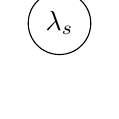
\begin{tikzpicture}[baseline=(char.base)]
\node(char)[draw,shape=circle]{$\lambda_s$};
\end{tikzpicture}\\
\cline{1-5}
\end{tabular}} \hspace{-0.3cm}\ar@{->}[r] &  \lambda_a} \\[0.6cm]
&\Rightarrow \,\, T \sim \text{Exponential}(\lambda_s-\lambda_a)\\[0.1cm]
{\footnotesize(\text{where $T$}} & {\footnotesize\text{ is the total time in the system)}}\\
\end{align*}

{\bf Normal Distribution:}\\[-0.6cm]
\begin{align*}
\bullet\quad X \sim \text{Normal}&(\mu,\sigma) \\[0.4cm]
\bullet\quad E(X) &= \mu \\[0.4cm]
\bullet\quad Var(X) &= \sigma^2 \\[0.4cm]
\bullet\quad (1-\alpha)100\% \text{ of the Normal}(\mu,\sigma) & \text{ distribution lies in } \mu \pm z_{\,\alpha/2}\,\,\sigma \\[0.4cm]
\bullet\quad \Pr(X > x) &= \Pr\left(Z> \frac{x-\mu}{\sigma}\right)\\[1cm]
\bullet\quad \Pr(Z < -z) &= \Pr(Z > z) \\[0.6cm]
\bullet\quad \Pr(Z > -z) &= \Pr(Z < z) = 1 -\Pr(Z>z) \\[1cm]
\bullet\quad \text{If} \,\,  X_1 \sim \text{Normal}(\mu_1,\sigma_1) \,\,  & \text{ and } \,\, X_2 \sim \text{Normal}(\mu_2,\sigma_2) \\[0.4cm]
\Rightarrow \quad  \text{ Sum: } \quad  X_1 + X_2 &\sim \text{Normal}\left(\mu_1+\mu_2,\,\sqrt{\sigma_1^2+\sigma_2^2}\,\right) \\[0.4cm]
\Rightarrow \quad  \text{ Difference: } \quad   X_1 - X_2 &\sim \text{Normal}\left(\mu_1-\mu_2,\,\sqrt{\sigma_1^2+\sigma_2^2}\,\right) \\[1cm]
\bullet\quad \text{For} \,\,  X_1,\ldots,X_n \sim \text{any distribution} & \text{ with } \mu = E(X) \text{ and } \sigma = Sd(X) = \sqrt{Var(X)}\\[0.4cm]
\Rightarrow \quad  \text{ Sample mean: } \quad  \,\overline{\!X} &\sim \text{Normal}\left(\mu,\,\frac{\sigma}{\sqrt{n}}\,\right) \quad \text{ if } n > 30
\end{align*}

\newpage


\section*{Useful Formulae: Page 4\\[0.3cm]}
{\bf Statistics and Standard Errors:}\\[0.1cm]
\begin{adjustwidth}{-2cm}{0cm}
\begin{tabular}{|c|c|c|c|c|}
\hline
&&&&\\[-0.1cm]
Parameter & Statistic & Standard Error & Samples & Details \\[0.3cm]
\hline
&&&&\\[-0.1cm]
$\mu$ & $\bar x$ & ${\displaystyle\frac{s}{\sqrt{n}}}$  & large / small & $\nu = n - 1$ \\[0.5cm]
\hline
&&&&\\[-0.1cm]
$p$ & $\hat p$ & \multirow{2}{*}{${\displaystyle\sqrt{\frac{\hat p\,(1-\hat p)}{n}}}$} & large & confidence \\[-0.1cm]
&&&&interval\\[0.3cm]
\cline{3-5}
&&&&\\[-0.1cm]
&  & \multirow{2}{*}{${\displaystyle\sqrt{\frac{p_0\,(1-p_0)}{n}}}$} & large & hypothesis \\[-0.1cm]
&&&&test\\[0.3cm]
\hline
&&&&\\[-0.1cm]
$\mu_1-\mu_2$ & $\bar x_1 - \bar x_2$ & \multirow{3}{*}{${\displaystyle\sqrt{\frac{s_1^2}{n_1}+\frac{s_2^2}{n_2}}}$} & large / small & ${\displaystyle \nu = \frac{(a+b)^2}{\frac{a^2}{n_1-1}+\frac{b^2}{n_2-1}}}$ \\[0.8cm]
&&&& ${\displaystyle a=\frac{s_1^2}{n_1}, \,\,\, b=\frac{s_2^2}{n_2}}$ \\[0.5cm]
\cline{3-5}
&&&&\\[-0.1cm]
&  & ${\displaystyle\sqrt{\frac{s_p^2}{n_1}+\frac{s_p^2}{n_2}}}$ & small & $\nu = n_1+n_2-2$ \\[0.5cm]
&&&& assuming \\[-0.2cm]
&& where\,\, ${\displaystyle s_p^2 = \frac{(n_1-1)\,s_1^2+(n_2-1)\,s_2^2}{n_1+n_2-2}}$  && $\sigma_1^2 = \sigma_2^2$ \\[0.5cm]
\hline
&&&&\\[-0.1cm]
$p_1-p_2$ & $\hat p_1 - \hat p_2$ & \multirow{2}{*}{${\displaystyle\sqrt{\frac{\hat p_1 \, (1-\hat p_1)}{n_1}+\frac{\hat p_2 \, (1-\hat p_2)}{n_2}}}$} & large & confidence\\[-0.1cm]
&&&&interval\\[0.5cm]
\cline{3-5}
&&&&\\[-0.1cm]
&  & ${\displaystyle\sqrt{\frac{\hat p_c\,(1-\hat p_c)}{n_1}+\frac{\hat p_c\,(1-\hat p_c)}{n_2}}}$ & large & hypothesis\\[-0.4cm]
&&&&test\\[0.2cm]
&&where\,\, ${\displaystyle \hat p_c = \frac{x_1+x_2}{n_1+n_2}}$&&\\[0.5cm]
\hline
\multicolumn{5}{c}{}\\[0.5cm]
\end{tabular}
\end{adjustwidth}
{\bf Confidence Intervals:}\\[-0.5cm]
\begin{align*}
\bullet\quad \text{Large sample:} \qquad \text{statistic } &\pm\,\, z_{\,\alpha/2}\,\times\,\text{standard error} \\[0.6cm]
\bullet\quad \text{Small sample:} \qquad \text{statistic } &\pm\,\, t_{\,\nu,\,\alpha/2}\,\times\,\text{standard error}
\end{align*}

\newpage

\section*{Useful Formulae: Page 5\\[0.3cm]}
{\bf Hypothesis Testing:}\\[-0.5cm]
\begin{align*}
\bullet\quad z &= \frac{\text{statistic}-\text{hypothesised value}}{\text{standard error}} \\[1cm]
\bullet\quad \text{p-value } &= \left\{
\begin{array}{rl}
2 \times \Pr(Z > |z|) & \text{if }  H_a: \, \mu \ne \mu_0\\[0.4cm]
\Pr(Z < z) & \text{if } H_a: \, \mu < \mu_0\\[0.4cm]
\Pr(Z > z) & \text{if } H_a: \, \mu > \mu_0\\
\end{array} \right.\\[1cm]
\bullet\quad F &= \frac{\text{larger variance}}{\text{smaller variance}} = \frac{s_{\text{larger}}^2}{s_{\text{smaller}}^2} \\[0.5cm]
 & \nu_1 = n_{\text{\,top}} - 1,\quad\, \nu_2 = n_{\text{\,bottom}} - 1 \\[1cm]
\bullet\quad \chi^2 &= \sum \frac{(o_i-e_i)^2}{e_i}\\[0.5cm]
\text{Goodness-of-fit: } \qquad &e_i = \text{total} \times p(x_i),\qquad \nu = n_f - 1- k \\[0.6cm]
\text{Independence: } \qquad &e_{ij} = \frac{r_i\,\times\,c_j}{\text{total}},\qquad \nu = (n_r - 1)\,\times\,(n_c - 1)\\[0.3cm]
\end{align*}
{\bf Information Theory:}\\[-0.5cm]
\begin{align*}
\bullet\quad h(x) &= - \log_2[p(x)] \\[0.6cm]
\bullet\quad H(X) &= E[h(X)] = \sum h(x_i)\,p(x_i) \\[1cm]
\bullet\quad l(x_i) &= \text{code-length for character } x_i \\[0.6cm]
\bullet\quad E(L) &= \sum l(x_i)\,p(x_i) \\[1cm]
\bullet\quad e &= \frac{H(X)}{E(L)} \\[1cm]
\bullet\quad &\sum 2^{-l(x_i)}  \le 1
\end{align*}


\end{document} 